Un webhook permite que servicios de terceros envíen actualizaciones en tiempo real a su aplicación. Las actualizaciones se activan por algún evento o acción por parte del proveedor de webhook, y se envían a su aplicación a través de solicitudes HTTP. Cuando recibe la solicitud, la maneja con una lógica personalizada, como enviar un correo electrónico o almacenar los datos en una base de datos.

\subsection{Webhooks Shopify}
Un webhook se puede usar para recibir notificaciones sobre eventos particulares en una tienda en linea. Después de suscribirse a un webhook, puede permitir que su aplicación ejecute código inmediatamente después de que ocurran eventos específicos en las tiendas que tienen su aplicación instalada, en lugar de tener que hacer llamadas API periódicamente para verificar su estado. Por ejemplo, puede configurar un webhook para activar una acción en su aplicación cuando un cliente crea un carrito de compras o cuando un comerciante cree un nuevo producto en su administrador de Shopify. Al usar las suscripciones de webhooks, puede hacer menos llamadas API en general, lo que garantiza que la aplicación sea más eficiente y se actualice rápidamente \cite{webhook}.
\vspace{0.8cm}

\begin{figure}[H]
  \centering
  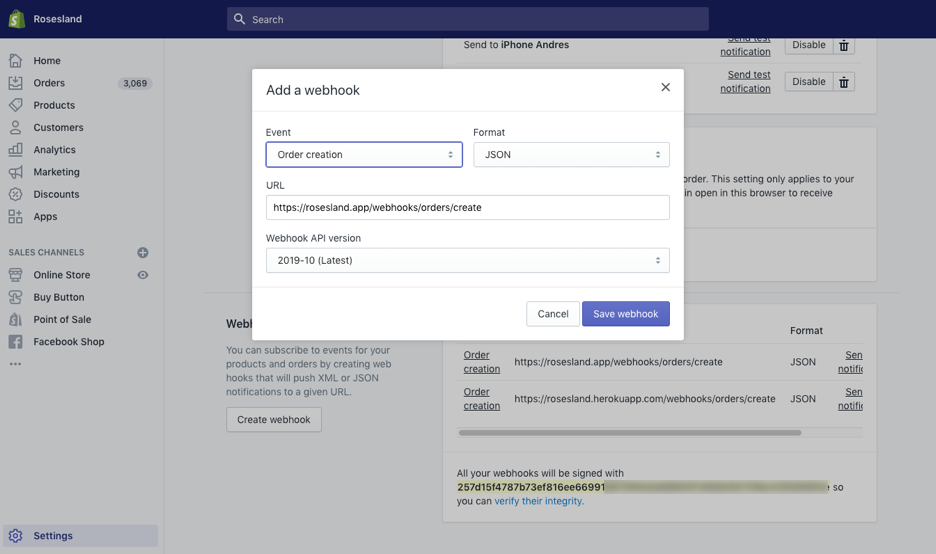
\includegraphics[width=1\textwidth]{webhook}
  \caption{Panel para crear webhooks en Shopify.}
\end{figure}

Después de configurar una suscripción de webhook, los eventos que especificó activarán una notificación de webhook cada vez que ocurran. Esta notificación contiene información JSON y encabezados HTTP que proporcionan contexto.

\newpage
\subsection{Configuración de webhook en Express.js}
En lugar de extraer información a través del API, los webhooks enviarán información a su punto final.
\vspace{0.8cm}

\lstinputlisting[style=ES6, caption=Ruta que capta el webhook lanzado desde Shopify]{code/webhook.js}